\section{CERN}

\paragraph{}The European Organization for Nuclear Research, known as CERN, is a premier particle physics laboratory located near Geneva, straddling the border between Switzerland and France. It operates the world's largest particle collider, the Large Hadron Collider (LHC), which consists of a 27-kilometer ring of superconducting magnets. The LHC is designed to collide protons at energies up to 14 teraelectronvolts (TeV)\cite{LHC_Description}. There are four large experiments at CERN: ATLAS, CMS, ALICE, and LHCb. The ATLAS experiment is designed to explore a broad range of physics phenomena, including the fundamental nature of matter, the forces that shape our universe, and the search for extra dimensions and particles that could make up dark matter \cite{ATLAS_Description}. The CMS experiment, similar in its broad objectives to ATLAS, aims to investigate the Standard Model of particle physics, including the detailed study of the Higgs boson and searching for clues beyond the Standard Model \cite{CMS_Description}. ALICE is specialized for studying the physics of strongly interacting matter at extreme energy densities, where a form of matter called quark-gluon plasma forms, which is believed to have existed shortly after the Big Bang \cite{ALICE_Description}. Lastly, the LHCb experiment focuses on understanding the differences between matter and antimatter by studying a type of particle known as the beauty quark, or b quark, and exploring what happened after the Big Bang that allowed matter to dominate over antimatter \cite{LHCb_Description}.

\section{Glance \& Fence}

\paragraph{}As already mentioned Glance is a system designed for database retrieval and manipulation, implemented using a set of components written in C++. Each component within Glance is dedicated to a specific feature, functioning as a separate program but sharing a common architectural framework. The system facilitates interaction between the user and various databases, enabling data retrieval and updates without requiring in-depth knowledge of SQL or database modeling. Glance's architecture allows it to communicate with web servers through the Common Gateway Interface (CGI), using the GNU CgiCC library to manage this interaction. It connects to databases via connectors that interface with specific database technologies, thereby streamlining the data handling process \cite{maidantchikGlanceProject}. For historical reasons, Glance (team) became the unofficial name of the international collaboration between UFRJ, through LPS, and CERN. The team of developers is majorly composed by UFRJ students who join a scientific initiation program on LPS, then eventually are invited for a two-year internship program at CERN. The average time a member spends in the Glance team is around four years. % do I need to prove?

\paragraph{} As described by Bruno Lange on \cite{fence-2015}, FENCE is a PHP framework structured using Object-Oriented Programming (OOP) principles. Its primary purpose is to facilitate the development of web systems through JSON configuration files. The framework is designed to allow classes of each system to extend abstract classes of FENCE. This setup is intended to enable the reuse of generic methods while also allowing the development of specific methods tailored to individual requirements. The framework encourages the implementation of the Model-View-Controller (MVC) pattern by providing various base classes that support data models, visualization classes, and controllers for functionalities. A critical feature of FENCE is its use of the DBOf class, which constructs the desired data models with their respective validations based on the provided configuration file.

\paragraph{} As already explored by Mário Simão on \cite{Simao2023Architectural} FENCE presented some key drawbacks that motivated the search for alternative solutions. Firstly, the design of FENCE resulted in high maintenance costs, reducing the time available for new application development. The installation process posed significant challenges, specially due to the necessity to fill many configuration files which were not documented. The process to gather these files usually included accessing the QA or production servers and navigating through the folders to find examples of such files. In this context, access to remote servers could also be another issue. Because of FENCE's layers coupling, when developing an interface component, for example, the database connector that would retrieve data to populate this interface should also be up and running, this implies in a development setup always connected to CERN's intranetwork accessible only through SSH (Secure Shell) tunnels. Running a ping test from Rio de Janeiro to CERN's server in Geneva

\begin{lstlisting}[language=bash]
$ ping lxplus.cern.ch
PING lxplus.cern.ch (188.185.24.20): 56 data bytes
64 bytes from 188.185.24.20: icmp_seq=0 ttl=42 time=179.759 ms
64 bytes from 188.185.24.20: icmp_seq=1 ttl=42 time=180.587 ms
64 bytes from 188.185.24.20: icmp_seq=2 ttl=42 time=179.565 ms
64 bytes from 188.185.24.20: icmp_seq=3 ttl=42 time=182.643 ms
\end{lstlisting}

\noindent
The average response time is 180ms, which would very often lead to unstable connections to the internal resources. This aspect is even more critical considering the development setup of the team, which was based on virtual machines hosted at CERN and accessed through Visual Studio Code using the Remote Development extension which, according to users on \cite{vscodeRemoteRelease}, may present frequent disconnections when the internet connection is not great.

\paragraph{} In addition to being difficult to learn for new developers, FENCE had other issues. One of the main problems was that it lacked documentation and had hidden dependencies. Another issue was that FENCE tried to solve common industry problems such as logging, ORM (object-relational mapping), and database connections in its own way. This approach made it harder to maintain FENCE in the long run compared to open-source alternatives that had dedicated support and documentation.
The micro-ORM FacTree within FENCE, for example, did not have any in-memory cache to optimize queries, resulting in many duplicated instances in memory and crashes when fetching large amounts of data such as for the Authorship. It also was not able to recursively instantiate classes with self-referencing foreign key in their tables.

\paragraph{}Finally, the lack of automated testing in both FENCE and its dependent systems led to unaddressed architectural flaws, poor design choices, and the accumulation of technical debt and issue backlog topping with 20 open issues on the issue tracker incluing tickets more than 1 year old. The high coupling with external resources further compounded the challenge of setting up a test environment.

\section{Super Search}

\paragraph{} As discussed by Souza Silva \cite{SouzaSilva2023Glance} the FENCE Super Search framework comprises a set of classes for crafting advanced search interfaces, segregated into two web views. The initial view, termed the Search Workspace \cite{fence-2015}, empowers users to build structured search criteria using logical operators. Users construct their queries by connecting nodes horizontally with \textbf{AND} operators and vertically with \textbf{OR} operators. This setup, however, reveals a significant limitation. \autoref{fence-ss-1} and \autoref{fence-ss-2} illustrate an attempt to \textbf{identify cables starting at point A and ending at point C, along with those starting at point B and ending at point D}. The process involves dragging and dropping nodes to form a query, with results subsequently presented in a tabular layout. To elucidate, consider the following statements in the context of a desired search:
\begin{equation}
\begin{split}
s_1: cable\_start = point A,
s_2: cable\_end = point C, \
\end{split}
\end{equation}
\begin{equation}
\begin{split}
s_3: cable\_start = point B,
s_4: cable\_end = point D \
\end{split}
\end{equation}
Ideally, the query to fetch the correct dataset would be:
\begin{equation}
query_1 = (s_1 \land s_2) \lor (s_3 \land s_4)
\end{equation}
\noindent
However, due to system limitations restricting connections to horizontal \textbf{AND}s and vertical \textbf{OR}s, this query becomes unachievable, highlighting a notable rigidity in the FENCE system's design.

\paragraph{}In practice, users often resort to an alternate query format, as depicted in \autoref{fence-ss-1}:
\begin{equation}
query_2 = (s_1 \lor s_3) \land (s_2 \lor s_4)
\end{equation}
\noindent
A closer analysis of $query_2$ reveals its inadequacy, as it includes undesired results, such as cases where both $s_1$ and $s_4$ are true. The differences between both queries is made explicit by the truth table. This led to the development of the new proposed search implementation aimed at overcoming these and other limitations inherent to the original system. 
\begin{center}
\begin{tabular}{|c|c|c|c||c|c|}
\hline
\( s_1 \) & \( s_2 \) & \( s_3 \) & \( s_4 \) & \( \text{query}_1 \) & \( \text{query}_2 \) \\
\hline
0 & 0 & 0 & 0 & 0 & 0 \\
0 & 0 & 0 & 1 & 0 & 0 \\
0 & 0 & 1 & 0 & 0 & 0 \\
0 & 0 & 1 & 1 & 1 & 1 \\
0 & 1 & 0 & 0 & 0 & 0 \\
0 & 1 & 0 & 1 & 1 & 1 \\
0 & 1 & 1 & 0 & 0 & 1 \\
0 & 1 & 1 & 1 & 1 & 1 \\
1 & 0 & 0 & 0 & 0 & 0 \\
1 & 0 & 0 & 1 & 0 & 1 \\
1 & 0 & 1 & 0 & 0 & 1 \\
1 & 0 & 1 & 1 & 1 & 1 \\
1 & 1 & 0 & 0 & 1 & 1 \\
1 & 1 & 0 & 1 & 1 & 1 \\
1 & 1 & 1 & 0 & 1 & 1 \\
1 & 1 & 1 & 1 & 1 & 1 \\
\hline
\end{tabular}
\end{center}


\paragraph{}The same issue can arise in the Membership context when searching, for example, for all members with primary affiliation is UFRJ and profession is Engineer plus all members with primary affiliation is PUC (Pontifícia Universidade Católica de São Paulo) and profession is PhD Student:
\begin{equation}
\begin{split}
s_1: affiliation = UFRJ,
s_2: profession = Engineer, \
\end{split}
\end{equation}
\begin{equation}
\begin{split}
s_3: affiliation = PUC,
s_4: profession = PhD Student \
\end{split}
\end{equation}

\paragraph{} Moreover, the presentation view's capabilities and styling are constrained by the parameters set in the JSON configuration file. While generally adequate, this setup struggles with \textbf{dynamic content} and complex behaviors. Additionally, the pagination system exhibits flaws, notably when dealing with large result sets, where operations like downloading, filtering, and sorting only consider the current page of results (and not the entire result set which may contain multiple pages). To bypass these limitations, users would often request the entire set of results to be displayed in one page, which often leads to unresponsive interfaces and page crashes when the browser run out of memory. 

\paragraph{} In the search results page, users could edit the layout by rearranging and hiding columns, applying additional client-side filters (lookup), and changing the pagination parameters (number of results per page). This layout could be saved, which is especially useful for searches performed daily. However, the save search feature relied on the browser's local storage, meaning that this information is lost when the cache expires. Finally, the lack of an API to expose search results to other systems was a decisive factor for the approval of the development of a new search solution. Despite these challenges, the FENCE Super Search became the most used data visualization tool in various systems across LHCb, ATLAS, and ALICE, serving thousands of users. This necessitates a careful transition to a new solution that retains existing functionalities while addressing these shortcomings. 


\begin{figure}[H]
    \centering
    \begin{minipage}[t]{.4\textwidth}
        \centering
        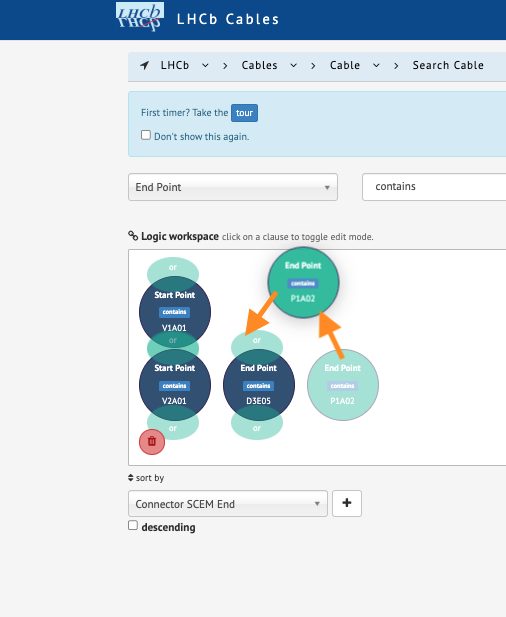
\includegraphics[width=\linewidth]{figuras/fence_search_1_sm.png}
        \caption{Query workspace.}
        \label{fence-ss-1}
    \end{minipage}
    \hfill
    \begin{minipage}[t]{.4\textwidth}
        \centering
        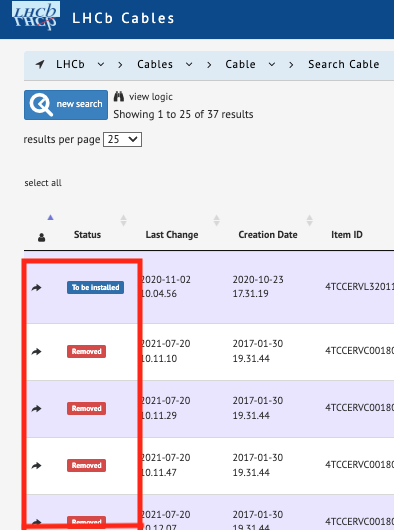
\includegraphics[width=\linewidth]{figuras/fence_search_2_sm.png}
        \caption{Fence search results.}
        \label{fence-ss-2}
    \end{minipage}
\end{figure}

\paragraph{} To provide a replacement for the SuperSearch, the main inspiration was Jira's Query Language \cite{jirajql}. Jira is a software tool developed by Atlassian that allows bug tracking, issue tracking, and agile project management. Jira Software supports different agile project management methodologies for software development, providing tools to estimate, report, and measure velocity with workflows designed to fit your frameworks. Since many years, it has been the officially supported issue tracker software at CERN. \cite{jirajql}

\paragraph{} As described by Dan Radigan \cite{jirajql}, Jira Query Language (JQL) is a flexible tool developed by Atlassian for searching issues in Jira. The key features of JQL (Jira Query Language) include advanced search capabilities, allowing users to perform complex searches using a structured query language; customizable queries, where users can create queries based on specific fields, operators, and values; and a syntax similar to SQL, making it intuitive for those with database query experience. The components of JQL consist of fields, which are the data points in Jira such as priority, status, and assignee; operators, which define the relationship between fields and values, with examples including ``=", ``!=", ``$\ge$", and ``$\le$"; and values, which are the actual data or criteria being queried. 

\paragraph{} Souza e Silva \cite{SouzaSilva2023Glance} describes similar definitions for the structured query language used on the new Super Search which was called Glance Search Library. On \cite{SouzaSilva2023Glance}, the Glance Query Language (GQL) is described as a pivotal aspect of the new architecture, being used on the server-side to convert query strings into SQL filters, forming a $WHERE$ clause by mapping query string elements (Eg.: table names, table columns, boolean operators) into SQL elements through a JSON configuration file. This design differs from FENCE's Super Search by limiting the JSON file's scope to mapping query string elements to database columns and caching settings, thus making the frontend interfaces independent of this file. 

\paragraph{} Using the same example from \cite{SouzaSilva2023Glance} to find \textit{all cables that start in point A and end in point C plus all cables that start in point B and end in point D} this would be written in GQL as 

\begin{multline*}
queryString_1: \text{(start\_point = PointA \textbf{AND} end\_point = PointC)} \\
\text{\textbf{OR} (start\_point = PointB \textbf{AND} end\_point = PointD)}
\end{multline*}

\noindent
And the GQL equivalent of the query that could be composed through FENCE's SuperSearch is \begin{multline*}
queryString_2: \text{(start\_point = PointA \textbf{OR} start\_point = PointB)} \\
\text{\textbf{AND} (end\_point = PointC \textbf{OR} end\_point = PointD)}
\end{multline*}

\noindent
With the GQL elements categorized in the table \ref{table:search-elements}.

\begin{longtable}{|p{0.25\textwidth}|p{0.5\textwidth}|p{0.25\textwidth}|}
\caption{Search elements}\label{table:search-elements} \\
\hline
\textbf{Element} & \textbf{Category} & \textbf{Identifier} \\ \hline
\endfirsthead

\multicolumn{3}{c}%
{{\bfseries \tablename\ \thetable{} -- continued from previous page}} \\
\hline
\textbf{Element} & \textbf{Category} & \textbf{Identifier} \\
\hline
\endhead

\hline
\endfoot

Start point & \textbf{Search Field} & $f_1$ \\
End point & \textbf{Search Field} & $f_2$ \\
= & \textbf{Search Operator} & $o_1$ \\
AND & \textbf{Search Conjunction} & AND \\
OR & \textbf{Search Conjunction} & OR \\
Point A, B, C, D & \textbf{Search Value} & $v_1, v_2, v_3, v_4$ \\
( & \textbf{Grouping Mark} & ( \\
) & \textbf{Grouping Mark} & ) \\
\hline
\end{longtable}


A \textbf{Search Statement} in GQL is a combination of a Search Field, Operator, and Value. For instance, from the queries, four statements are derived: $s_1: f_1 \frown o_1 \frown v_1$, $s_2: f_2 \frown o_1 \frown v_3$, $s_3: f_1 \frown o_1 \frown v_2$, and $s_4: f_2 \frown o_1 \frown v_4$ where ``X" $\frown$ ``Y" $\frown$ ``Z" denotates the concatenation of the SearchField ``X", a space character, the SearchOperator ``Y", another space chacters plus the SearchValue ``Z". Rewriting the query strings as a funcion of the statements $queryString_1$: ($s_1$ $\land$ $s_2$) $\lor$ ($s_3$ $\land$ $s_4$) and $queryString_2$: ($s_1$ $\lor$ $s_3$) $\land$ ($s_2$ $\lor$ $s_4$). The design of GQL, decoupled from interface and infrastructure constraints, ensures that both queries are valid, resolving the limitations encountered in the FENCE system where $queryString_1$ could not be created.

\paragraph{} With GQL, it is already possible for users to perform a search by typing the query string in a text input. However, in order to assist users with the query formulation and prevent syntax errors, an interface component to handle advanced boolean searches had to be built. Because users were very familiar with FENCE's SuperSearch as it was in use for many years, the new solution should resemble the query composition mechanism to reduce the learning curve. This means going against most UX research, which tends to favor simpler search interfaces, as discussed on \cite{Nielsen2001SearchVisible}. In this article, titled ``Search: Visible and Simple", the author gives some general guidelines on how to handle search in a web application. The author emphasizes the importance of maintaining a straightforward and accessible search interface in web applications. This approach is grounded in the observation that users generally prefer and perform better with simpler search mechanisms. Complex or advanced search interfaces, while potentially powerful, can often lead to user confusion and frustration, especially for those not skilled in intricate query formulation. The article suggests that a basic search box is usually sufficient for most users’ needs, and its prominent placement, preferably on the homepage, enhances usability. Moreover, the design should focus on optimizing first-time search success, as users' likelihood of finding desired results diminishes with each subsequent search attempt. The author argues that, while advanced search capabilities may have their place, especially in specialized applications, they should not overshadow the simplicity and accessibility of the primary search function. This perspective challenges the idea of replicating the complex mechanisms of FENCE's SuperSearch, proposing instead that a more user-friendly approach, with an emphasis on simplicity and visibility, could lead to a more effective and efficient search experience for the majority of users.

\paragraph{} At the same time, other publications, such as ``How to Design Advanced Search Interface – Step by Step" by Abhijit Rawool \cite{RawoolAdvancedSearch}, acknowledge the necessity of an advanced boolean search interface and give general guidelines for improved usability. Rawool argues that while advanced search might not be essential for all applications, it plays a crucial role in complex systems like enterprise-level applications. He suggests a thoughtful approach to implementing advanced search, emphasizing that it should only be used when simple search fields are insufficient. Rawool recommends starting with a quick search interface and then providing an option for advanced search, echoing the sentiment that basic search meets most users' needs. However, when more detailed searches are required, advanced search interfaces become valuable. He advises careful consideration of the user interface (UI), suggesting that the advanced search form should be hidden initially and only made visible when the user opts for more detailed search criteria. In designing advanced search forms, Rawool highlights the importance of user effort in interpreting these interfaces. Each field in the advanced search should be clearly labeled and intuitive to use, minimizing the cognitive load on users. Furthermore, he advocates for including clear or reset buttons, allowing users to easily start their search over, which is particularly helpful given the larger number of fields in advanced search forms. Additionally, Rawool addresses the potential clutter of numerous search fields. He proposes the ``Add Fields" feature, where users can customize their search by adding additional fields as needed, keeping the interface clean and user-focused. This approach not only declutters the interface but also empowers users to tailor their search experience according to their specific needs.

\paragraph{} These publications played a crucial role in the decision to build a modular search interface based on web components. A web component is essentially a self-contained, reusable module in a web application. It encapsulates HTML, CSS, and JavaScript, allowing developers to create custom, encapsulated HTML tags for use in web pages and apps. This design choice gives developers the flexibility to customize the interface, allowing them to add necessary features and remove those that are not needed for a particular use case. Another important decision was to combine the query composition area with the search results display. This was based on the observation that users often perform searches without applying any filters, just to see a full list of entities (eg.: loading the information of all institutes). By merging these two interfaces, the system can cache this list, giving a snappier feel to the user. The final decision involved adding a quick lookup search (also known as simple search) on the homepage and fixed in the navigation bar. This was influenced by the recommendations from \cite{Nielsen2001SearchVisible} and \cite{RawoolAdvancedSearch}, which emphasize the importance of having an always visible search feature. This is particularly useful for instances where a user wants to search for a specific entity, such as a member searching for their institution. In such cases, the simple search will accept a string as input and return the link for the entity's profile in the system.


\paragraph{} In order to build a component based web interface it is necessary to map the fundamental components and how they will interact with each other.  An Event Storming workshop was used to map such components as described by Michelly Teixeira on \cite{michelly} . This workshop was a collaborative effort to clarify the business logic behind the search functionality and model its components effectively.


\paragraph{} Event Storming helped the team map the search process using sticky notes on a virtual board, leading to the identification of domain events, user actions that triggered these events, and their organization into a timeline. The session began with brainstorming to define relevant events for the user and system, which were then associated with user or system actions that triggered them. The exercise provided insights into the actions, entities, and actors involved in the search process. Subsequent meetings analyzed these insights to define the search interface components, detailing the properties each component should access and manage, resulting in two main views: the Filters View and the Results View. A state management pattern library was chosen to manage communication between components, centralizing the state to handle the search interface more effectively. The final result documented each component's role in generating commands and consuming events. Interface mockups were created to visualize the web components, exploring the possibility of merging search inputs and results into a single view for a more responsive user experience.


\section{The LHCb Membership}
\paragraph{} As already discussed in the introduction, the LHCb is a geo-distributed scientific collaboration that specializes in investigating the slight differences between matter and antimatter by studying a type of particle called the ``beauty quark" \cite{LHCb_Description}. The LHCb Membership is a system used to manage the collaboration participants, automatizing bureaucratic processes and enforcing the rules defined in the LHCb Constitution \cite{LHCbConstitution}. The main users of the LHCb Membership System are the LHCb Management, the Editorial Board (EB), the Membership Committee, the Secretariat and Institute and Country Representatives. As of February 2024 LHCb has 97 universities and research centers associated from 23 countries and 1656 members.

\subsection{Collaboration organization}

\paragraph{} The LHCb Constitution \cite{LHCbConstitution} defines a series of roles in the collaboration. The most relevant roles for the Membership context are described below.

\paragraph{} The LHCb Management serves as the executive body responsible for the operation of the detector, its upgrades, and physics analysis. It represents the LHCb Collaboration to external entities and comprises the Spokesperson, Deputy Spokespersons, Technical Coordinator, and Resources Coordinator. Advised by the Technical Board, Operations Planning Group, and Physics Planning Group, the LHCb Management makes daily decisions and communicates relevant issues to the Collaboration Board (CB).

\paragraph{}Major decisions by the Management are reported to the Plenary Meeting and then to the CB for endorsement. In urgent situations, where decisions cannot wait for a CB meeting, the Chairperson of the CB is consulted, and the decision is reviewed at the subsequent CB meeting. The Management maintains open communication with CERN Management and organizes resources, preparing the LHCb budget for presentation to the CB and the Resources Review Board. Additionally, the Management nominates Project Leaders and the Operations Coordinator, subject to CB approval, and may establish ad hoc Working Groups, recommending Conveners to the CB.

\paragraph{}The Spokesperson, as head of the LHCb Management, officially represents the collaboration and is the primary contact between LHCb, CERN Management, and the LHCC. Elected by the CB, the Spokesperson holds ultimate responsibility for the experiment and has authority over the production and dissemination of physics results, reporting directly to the CB.

\paragraph{}Deputy Spokespersons, nominated by the Spokesperson and ratified by the CB, represent the Spokesperson in their absence and may take on specific responsibilities, with any significant delegations being reported to the CB. They are non-voting, ex officio members of the CB, Operations Planning Group, Technical Board, and Physics Planning Group, and their term ends with the Spokesperson's term.

\paragraph{}The Resources Coordinator, nominated by the Technical Coordinator with the Spokesperson's agreement and ratified by the CB, oversees financial planning. This includes establishing annual budgets and expenditure reports for the CB and LHCb Resources Review Board, monitoring payments, and managing the implementation procedure for late M\&O (maintenance and operation) fund contributions. The Resources Coordinator reports to the Technical Coordinator and the CB and is an ex officio member of both the Technical Board and the CB. These are heavy users of the Membership, as the M\&O fee paid by the universities and research centers is a function of their number of members. 

\paragraph{}The LHCb Editorial Board (EB) oversees the collaboration's publication standards, with members appointed by the Spokesperson and ratified by the Collaboration Board. Terms are two years, with staggered renewals for continuity. The EB manages the review process for publications, ensuring the collaboration's input is incorporated and the proper authors list is used. In case of disputes, decisions are made by the EB Chairperson, Physics Coordinator, and Spokesperson. The EB also maintains a database of official LHCb results and materials.

\paragraph{}The LHCb Authorship rules in \cite{LHCbConstitution} state that collaborators earn the right to sign physics papers by contributing to the experiment, including detector construction, real-time analysis, online projects, computing projects, data taking, calibration, or data processing. Institutes must engage in service tasks as well. Authorship begins six months after joining LHCb and extends for 12 months post-membership. Annually, institutes submit a default author list, influenced by their M\&O budget share. PhD students are not bound by this quota. Retired active members can gain Emeritus status, allowing them to sign papers without M\&O and service obligations, subject to annual confirmation and support from LHCb coordinators or the Spokesperson. Authors can opt out of signing a paper, and exceptions to these rules are handled by the Editorial Board Chairperson, the Spokesperson, and the relevant institute leader, with a possible appeal to the Spokesperson. The Editorial Board reports to the CB on exception requests. The list is created and managed by the Authorship system which is a part of the Membership.

\paragraph{}LHCb membership comprises two types: Institute and Individual. Institute membership concerns CB treatment, while Individual membership involves status and access rights. The Membership Committee, set up by the CB and Management, reviews applications and participation in essential tasks. The Committee is formed after each CB chair election and reports to the CB.

\paragraph{} New institutes express interest to join LHCb through a letter, followed by a meeting with the Spokesperson and CB Chairperson to draft a detailed application, including contributions and service task plans. The Membership Committee reviews the application, and the institute presents its contributions to the CB. Admission requires two-thirds CB vote support. If positive, the institute is included in the M\&O sharing and recognized by the LHC Resource Review Board. Institutes may also become Associated or Technical Associated Members.\paragraph{} Individual membership for members from existing LHCb institutes is managed by their institute leader, who also notifies the LHCb secretariat of departures.  Significant growth in an institute's size is communicated to the CB Chair and Spokesperson, detailing resource and contribution changes for evaluation by the Membership Committee and CB.

\paragraph{} Associated Membership is for institutes contributing to specific projects, hosted by an LHCb institute, and responsible for long-term maintenance. They don't have a CB vote but are represented by their host and are eligible for LHCb authorship.  Technical Associated Membership is for institutes contributing to detector or computing projects, without access to data or LHCb authorship, but they may participate in hardware and software development.

\paragraph{} Individual membership categories vary by status and access rights, with different levels of affiliation and authorship conditions. Full members have full access and primary affiliation, while Technical and Software Associates have restricted access tied to specific projects. Affiliates, such as theorists, have short-term full access, with potential authorship on individual papers. Access rights and full membership are subject to approval and cannot be granted to individuals from Technical Associated Member institutes. M\&O contributions are expected from full member academics and postdocs.

\paragraph{} The LHCb Secretariat plays a key role in the collaboration management. Once a member or institution is accepted in the collaboration, they operationalize their registration procedures.  They also monitor the affiliation statuses and provide support with CERN's bureaucratic processes.

\paragraph{} Therefore, the major roles for the Membership context are summarized in table \ref{table:LHCbRoles}.


\begin{longtable}{|p{0.4\textwidth}|p{0.55\textwidth}|}
\caption{Major roles in LHCb for the Membership}\label{table:LHCbRoles} \\
\hline
\textbf{Role} & \textbf{Responsibilities and Characteristics} \\ \hline
\endfirsthead

\multicolumn{2}{c}%
{{\bfseries \tablename\ \thetable{} -- continued from previous page}} \\
\hline
\textbf{Role} & \textbf{Responsibilities and Characteristics} \\
\hline
\endhead

% Now, list each role with its responsibilities
Spokesperson and Deputy & Represents the collaboration, primary contact between LHCb and CERN Management, ultimate responsibility for the experiment. Elected by the CB. \\
\hline
Technical Coordinator & Part of the LHCb Management, advises on technical aspects of the detector and its upgrades. \\
\hline
Resources Coordinator & Oversees financial planning, monitors payments, and manages the M\&O fund contributions. Reports to the Technical Coordinator and the CB. \\
\hline
Project Leaders & Nominated by the Management, subject to CB approval, lead specific projects within the collaboration. \\
\hline
Editorial Board (EB) & Oversees publication standards, manages review process for publications, and maintains a database of official LHCb results. Members appointed by the Spokesperson and ratified by the CB. \\
\hline
Membership Committee & Reviews applications for Institute and Individual membership, reports to the CB. Formed after each CB chair election. \\
\hline
Institute Members & Involved in CB treatment, participate in M\&O sharing, can be Full, Associated, or Technical Associated Members. \\
\hline
Individual Members & Vary by status and access rights, managed by institute leader, include Full members, Technical and Software Associates, and Affiliates. \\
\hline
LHCb Secretariat & Manages registration procedures, monitors affiliation statuses, provides support with CERN’s bureaucratic processes. \\
\hline
Administrators & Glance developers and project managers \\
\hline
\end{longtable}




\subsection{Business requirements}
\paragraph{} The LHCb Membership System is used to manage the affiliations of \textbf{Member}s and \textbf{Institute}s (universities and research centers) with LHCb. Institutes, upon joining LHCb, open a \textbf{Participation} (which can be official, associated, technical, only for authorship and other types) with a period.  The Membership integrates with CERN's Human Resource (HR) systems and provides information to other applications that need to consume the list of Members. Members are affiliated with Institutes through one or multiple \textbf{Employment}s. The Employment includes information such as the affiliation type (primary or secondary), the \textbf{Profession}, flags to determine whether a member is entitled to authorship and counts for M\&O and the affiliation period. Members can also be assigned to special roles (Spokesperson, Team Leader, Safety Officer and more) which are called \textbf{Appointment}s. An Appointment may have an associated \textbf{Country} (eg.: for Country Representative), Institute (eg.: for Team Leader) or \textbf{Physics Working Group}. For the Authorship, there can be \textbf{Exception}s which are Members added to a specific \textbf{Paper}'s list of authors due to their exceptional contributions or members who requested to be removed from the paper. It is also possible to add \textbf{External Author}s affiliated with LHCb Institutes or \textbf{External Institute}s. \textbf{Funding Institution}s can also be acknowledged on a paper basis due to financial \textbf{Grant}s provided to Members or Institutes.

\paragraph{} The LHCb Membership Version 1 was essentially a CRUD system, providing digital forms for users to fill in the registration details for the entities just listed and search interfaces to retrieve these instances' information. It also sent periodic notifications using job schedulers. During the rewrite, all the CRUD functionality had to be implemented in the new stack, but the team used the opportunity to better understand how the processes in the collaboration worked in real life  and tailor the system to better fit the user needs. The table \ref{table:lhcb_membership_requirements}, lists the Membership System requirements. The requirements marked with an asterisk (*) will be enriched in the Workflow Project, aimed at transitioning real-life approval workflows into the Membership system. This transition involves multiple roles collaboratively reviewing and signing off on a document, ultimately leading to a specific outcome or action being recorded in the Membership database. Requirements marked with ``**" could only be implemented in the new stack, as FENCE's rigid architecture made them unfeasible.


\begin{longtable}{|p{0.05\textwidth}|p{0.45\textwidth}|p{0.4\textwidth}|}
\caption{LHCb Membership System Requirements and Role Access} \label{table:lhcb_membership_requirements}\\
\hline
\textbf{\#} & \textbf{Requirement Title \& Description} & \textbf{Roles Access} \\
\hline
\endfirsthead

\multicolumn{3}{c}%
{{\bfseries \tablename\ \thetable{} -- continued from previous page}} \\
\hline
\textbf{No.} & \textbf{Requirement Title \& Description} & \textbf{Roles Access} \\
\hline
\endhead


\hline
\endlastfoot

1 & Display User Info: Users can view other Member's information. & Basic User, Administrator, Secretariat \\
\hline
2* & User Registration: Administrators can insert new Members with specific rules. & Administrator \\
\hline
3 & Member Edition: Allows editing of Member details. & Administrator \\
\hline
4 & User History Tab: Users can view their profile updates. & Basic User, Administrator, Secretariat \\
\hline
5 & Search User: Users can search for other Members. & Basic User, Administrator, Secretariat \\
\hline
6 & Institute Insertion: Administrators can add new Institutes with specific rules. & Administrator, Secretariat \\
\hline
7 & Institute Edition: Allows updating Institutes' basic info. & Administrator, Secretariat \\
\hline
8 & Institute Details: Viewing of Institutes' basic and Employment info. & Basic User, Administrator, Secretariat, Team Leader \\
\hline
9 & Institute History Tab: Users can see updates to Institutes. & Basic User, Administrator, Secretariat \\
\hline
10 & Search Institute: Enables searching for Institutes. & Basic User, Administrator, Secretariat \\
\hline
11 & Employment End Notification: Notifies specific roles before Employment ends. & Administrator, Secretariat \\
\hline
12* & Add Employment: Administrators and Secretariat can add Employment for users with rules. & Administrator, Secretariat \\
\hline
13* & Update Employment: Administrators and Secretariat update Member's Employments. & Administrator, Secretariat \\
\hline
14 & Employments Tab: Viewing of user's Employment records. & Basic User, Administrator, Secretariat, Team Manager \\
\hline
15** & Display Statistics for Institutes: Visualize Institute statistics. & Basic User, Administrator, Secretariat \\
\hline
16** & Display Statistics for Countries: Country Representatives can view Country statistics. & Administrator, Secretariat, Country Representative \\
\hline
17 & Public Page for Authors List: Access to LHCb authorship list for a given date for unlogged users. & Public \\
\hline
18 & Upcoming Employment Notification: Advance notification about upcoming Employments. & Administrator, Secretariat \\
\hline
19 & Institute Change Notification: Notifies Team Leaders about Institute Participation changes. & Administrator, Secretariat, Team Manager \\
\hline
20 & Notification of Legacy Members: Semi-annual check for possible duplicates of old Members. & Administrator, Secretariat \\
\hline
21 & Summary M\&O Report: Access to summary reports for specific roles. & Administrator, Secretariat, Resource Coordinator, Team Manager \\
\hline
22 & Detailed M\&O Report: Detailed M\&O reports with access for specific roles. & Administrator, Secretariat, Resource Coordinator, Team Manager \\
\hline
23 & Add Warning to Update Appointment End Date: Synchronization or warning for appointment end dates. & Administrator, Secretariat \\
\hline

\end{longtable}

\paragraph{} Differently from the Membership System that already had a working version and a set of requirements reasonably fulfilled, the Authorship system requirements were not clear and the only document available was the LHCb constitution \cite{LHCbConstitution} that lacks in details and do not cover corner cases. To gather the Authorship system requirements, the developers organized a series of customer interviews, which, based on \cite{CustomerInterview}, are a qualitative research method aimed at understanding users' needs, preferences, experiences, and challenges with a software product. This process involves planning the interview objectives, recruiting representative participants, conducting interviews with open-ended questions, analyzing the responses to identify common themes, and using the insights to guide development decisions. The practice ensures a user-centric design, as it provides direct feedback from users or potential users, helping to validate assumptions, identify pain points, and inform feature prioritization. 

\paragraph{} This effort resulted in an internal document describing the rules for a Member to be considered an Author:
\begin{itemize}
    \item The Member should have the ``full member'' membership access status;
    \item The current Employment Profession is neither Master Student nor Bachelor Student;
    \item The Member has an active Employment entitled to authorship OR the last Employment entitled to authorship ended in one year at most before the reference date;
    \begin{itemize}
        \item The second condition is taken into account for Members that fully terminated their LHCb membership and also for Members that switched from an affiliation entitled to authorship to an affiliation not entitled to authorship. This way, the system ensures fairness by applying the 1 year grace period to both active and inactive Members;
    \end{itemize}
    \item The sum of the periods of Employments entitled to authorship is $\geq 6$ months (180 days);
    \begin{itemize}
        \item Every Employment entitled to authorship started before the reference date is counted (even the ones ended more than 1 year ago);
        \item Overlapping primary and secondary Employments are not counted twice;
        \item By default, an Employment is entitled to authorship when the profession is one of the following: Emeritus, PhD Engineer, Post Doc, PhD Student, or Senior.
    \end{itemize}
\end{itemize}

\noindent
 Alongside the more precise authorship rules, the system requirements were gathered and are listed in the table below. An \textbf{Authorship} list can be compiled for a given date of for a given paper. Exceptions are only added to papers' authors lists. 

\begin{longtable}{|p{0.05\linewidth}|p{0.25\linewidth}|p{0.65\linewidth}|}
\caption{Authorship System requirements} \\
\hline
\textbf{\#} & \textbf{Title} & \textbf{User Story \& Notes} \\
\hline
\endfirsthead

\multicolumn{3}{c}%
{{\bfseries Table \thetable\ continued from previous page}} \\
\hline
\textbf{\#} & \textbf{Title} & \textbf{User Story \& Notes} \\
\hline
\endhead

\hline
\endfoot

\hline
\endlastfoot

1 & Display Paper Interface & A user wants to visualize all papers and their information in a table. This includes paper status, identifier, title (supporting latex), number of authors, exceptions, reference date, and admin functions (export, delete, edit). \\
\hline
2 & Search Paper & A user wants to search already created paper by paper title. \\
\hline
3 & Download Paper & A user wants to export the authorship list in various formats: arXiv latex, InSpire xml, simple latex, PDF, and lists grouped by institute. \\
\hline
4 & Remove Paper & An admin wants to remove a non-published paper. \\
\hline
5 & Manage Paper & An admin wants to manage an ``on going" paper, with capabilities to remove/add authors, change paper status to published, and add institutes. \\
\hline
6 & Exceptions Summary & An admin wants to visualize a summary of the authors and institutes added or removed from the authorship list. \\
\hline
7 & External Authors & An admin can add authors from outside the LHCb collaboration, requiring details like initials, author name (in English), latex name, Inspire, ORCiD, and institute affiliations. \\
\hline
8 & External Institutes & If the author is from an external institute, it can be added with details like institute name, city, country, and main affiliation status. \\
\hline
9 & Create Paper & An admin can create a new paper, specifying details like paper title (supporting latex), reference date, a unique custom paper identifier, and an optional CDS link. The default paper identifier format is detailed. \\
\hline
10 & Preview Authorship List & A user wants to preview the list ordered by last name, with the ability to filter by institute and clearly see all external members/institutes added or removed. \\
\hline
11 & Authorship for a given date & A user wants to preview the authorship list for a given date \\
\hline
12 & Download Authorship for date & A user wants to download the authorship list for a given date \\
\hline
13 & Register Funding Agency & An admin or Secretariat wants register a Funding Agency \\
\hline
14 & Register/Manage Grant & An admin or Secretariat wants to register/update/delete a financial Grant provided by a Funding Agency to a Member or Institute \\
\hline
15 & Register/Manage Grant & An admin or Secretariat wants to register/update/delete a financial Grant provided by a Funding Agency to a Member or Institute \\
\hline
16 & Acknowledge Grant & The EB Chair wants to acknowledge a Grant in a Paper's authors list \\

\end{longtable}

\paragraph{} With the requirements gathering process concluded, the author started to develop mock interfaces, which were again validated with the EB. This marks the start of the migration to a new software architecture in the LHCb Glance systems.

\paragraph{} The Authorship was very modified a second time at the beginning of 2023 due to the Russia-Ukraine conflict which, in February 2022, escalated significantly when Russia launched a full-scale invasion of Ukraine, marking a substantial increase in hostilities and leading to widespread international condemnation, additional sanctions against Russia, and a humanitarian crisis. The conflict has had far-reaching implications, including economic disruptions, an energy crisis in Europe, and concerns about broader regional or global security implications. In response to the complex dynamics and personal convictions stemming from the conflict, the EB decided to first allow authors to hide their affiliations on the authorship lists. This decision was made to accommodate authors who wished to dissociate themselves from their institutions, particularly those affiliated with Russian institutes, due to disagreements with their institution's stance or the broader political situation. Subsequently, the EB also permitted authors to completely remove their names from authors lists including Russian institutes if they chose to, reflecting a stance of personal or ethical disagreement. This necessitated modifications to the authorship algorithm to support these requests, ensuring that authors could exercise their choices regarding affiliation visibility and participation in a manner consistent with their principles and the evolving situation. The final directive issued by the Editorial Board (EB) implied in the exclusion of all Russian institutes from the author lists, reinforcing LHCb's stance of condemning the actions undertaken by Russia. 



\subsection{Workflow Project}
\label{subsec:workflow_project_cap_2}
\paragraph{} While exploring the possible architectural patterns for the new refactor projects, the developers came across the Ubiquitous Language and Domain Driven Design (DDD) concepts.  Eric Evans, in his book ``Domain-Driven Design"  \cite{evans2003domain}, defines a software development approach centered around modeling software to faithfully reflect the core concepts and rules of a specific domain. This philosophy, deeply rooted in understanding the domain itself, emphasizes building software that aligns with business needs and adapts to complexity. The fundamental pillar of Evans' DDD rests on ubiquitous language, a shared vocabulary established by developers and domain experts. This common language ensures everyone operates on the same page, reducing communication gaps and fostering collaboration. It's through this language that the domain model emerges, a conceptual representation of the core entities, their relationships, and the domain's inherent rules.  

% Maybe I'll need something to support this user pain thing
\paragraph{} A significant challenge identified with Membership V1 was its constrained functionality within collaboration procedures, particularly evident in the newcomer registration process. This limitation is illustrated in the flowchart referenced in Figure \ref{fig:registration_old}. The flowchart delineates tasks executed by newcomers in yellow and those undertaken by the LHCb Secretariat in orange. A holistic analysis reveals the LHCb Membership's restricted application and its susceptibility to errors, primarily due to the Secretariat's potential need to manually input information from numerous PDF forms into the system. Also, the redundancy of data entry is another critical issue; information solicited through the LHCb registration form PDF, shown in Figure \ref{fig:lhcb_registration_form_pdf}, often duplicates data already present in CERN's HR system. This duplication not only burdens users with repetitive data entry tasks but also heightens the risk of data inconsistencies across different platforms.

\begin{figure}[H]
    \centering
    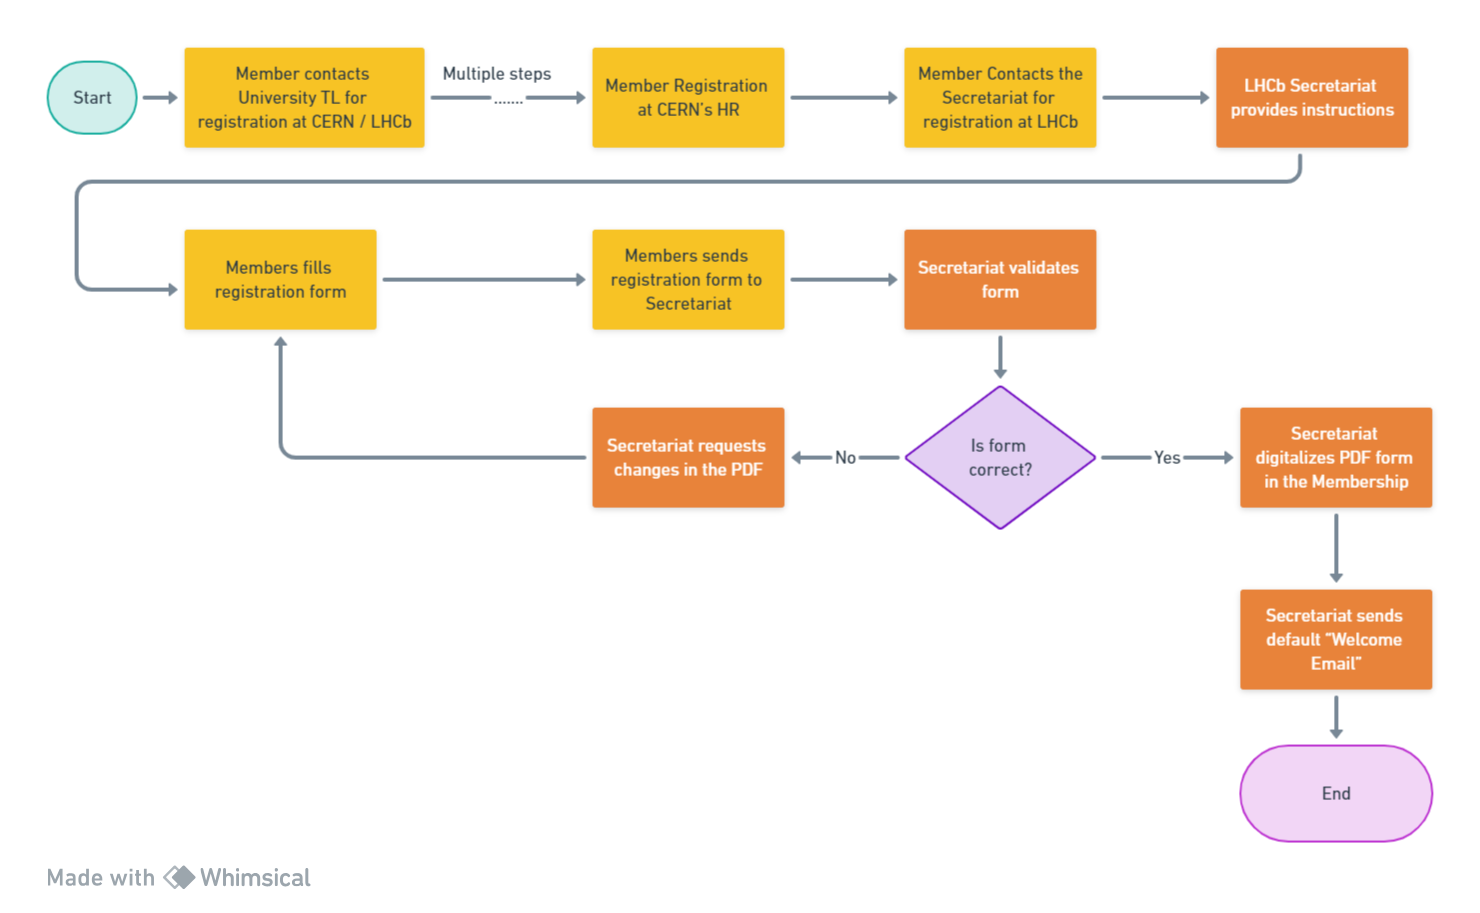
\includegraphics[width=1\linewidth]{figuras/newcomer_wf.png}
    \caption{LHCb newcomer registration procedure.}
    \label{fig:registration_old}
\end{figure}

\begin{figure}[H]
    \centering
    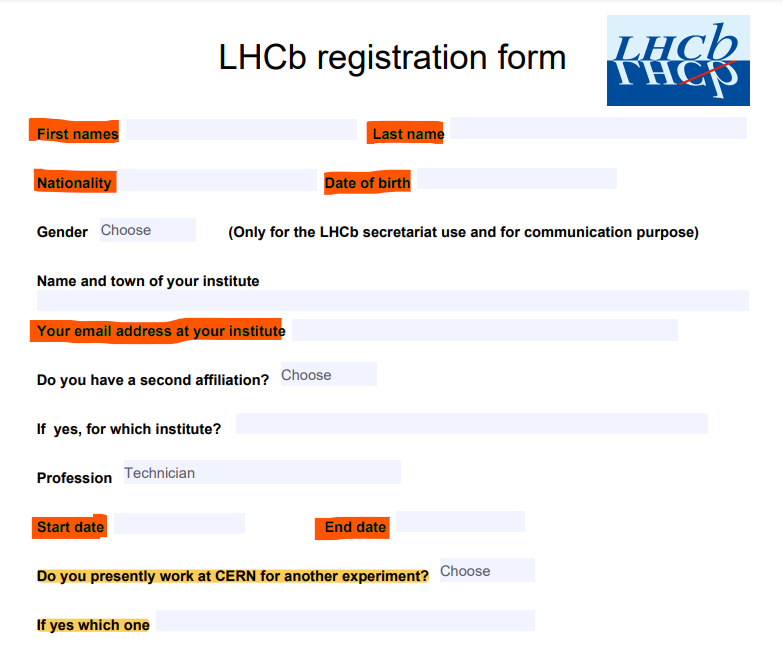
\includegraphics[width=0.6\linewidth]{figuras/lhcb_form.png}
    \caption{LHCb newcomer registration PDF form. All information highlighted in red is already present in CERN's HR database once this form is filled by the newcomer.}
    \label{fig:lhcb_registration_form_pdf}
\end{figure}

\paragraph{} In contrast to traditional CRUD systems like Membership V1, which primarily focus on the basic operations of data persistence and manipulation DDD emphasizes the modeling of the domain's intricacies and its fundamental principles, facilitating the creation of software that is highly congruent with business objectives and capable of evolving alongside them. Specifically, in the context of the workflow depicted in Figure \ref{fig:registration_old}, DDD advocates for more atomic actions. An example would be implementing a feature that allows the Secretariat to directly reject a registration form with a single click, which would then automatically trigger an email notification to the newcomer, prompting them to amend their submission. Additionally, a scheduled task could regularly check CERN's HR systems for new registrations, automatically initiating the LHCb registration process by firing email notifications with the necessary instructions through a static page on the Membership platform. These enhancements, derived from discussions with key users of the Membership system, aim to streamline and enrich the user experience. Further, additional workflows have been identified and mapped to extend the system's functionality, including the modification of Employment profession, the extension of Employment periods, and the creation of new Employment records. 

\paragraph{}These enhancements highlight the transformative capacity of Domain-Driven Design (DDD) in redefining system architecture, ensuring it mirrors the details of real-world business operations and addresses the needs of its users effectively. Furthermore, this approach has motivated the creation of software tools capable of monitoring the lifecycle of entities through approval workflows. The conceptual diagram, referenced in Figure \ref{fig:cap_2_workflow_draft}, provides a view of the proposed workflow tracking mechanism. This model documents all conceivable \textbf{States} (represented by circles) an entity might occupy, alongside \textbf{Transitions} (depicted by arrows) between these States. A Transition is initiated once all requisite \textbf{Conditions} are met. The envisioned Workflow Tracker would monitor \textbf{Events}, marking a Condition as fulfilled upon the occurrence of a corresponding Event. This system is designed to inform an Entity of its current State, potential subsequent States, and the Conditions necessary for progression.

\begin{figure}[H]
    \centering
    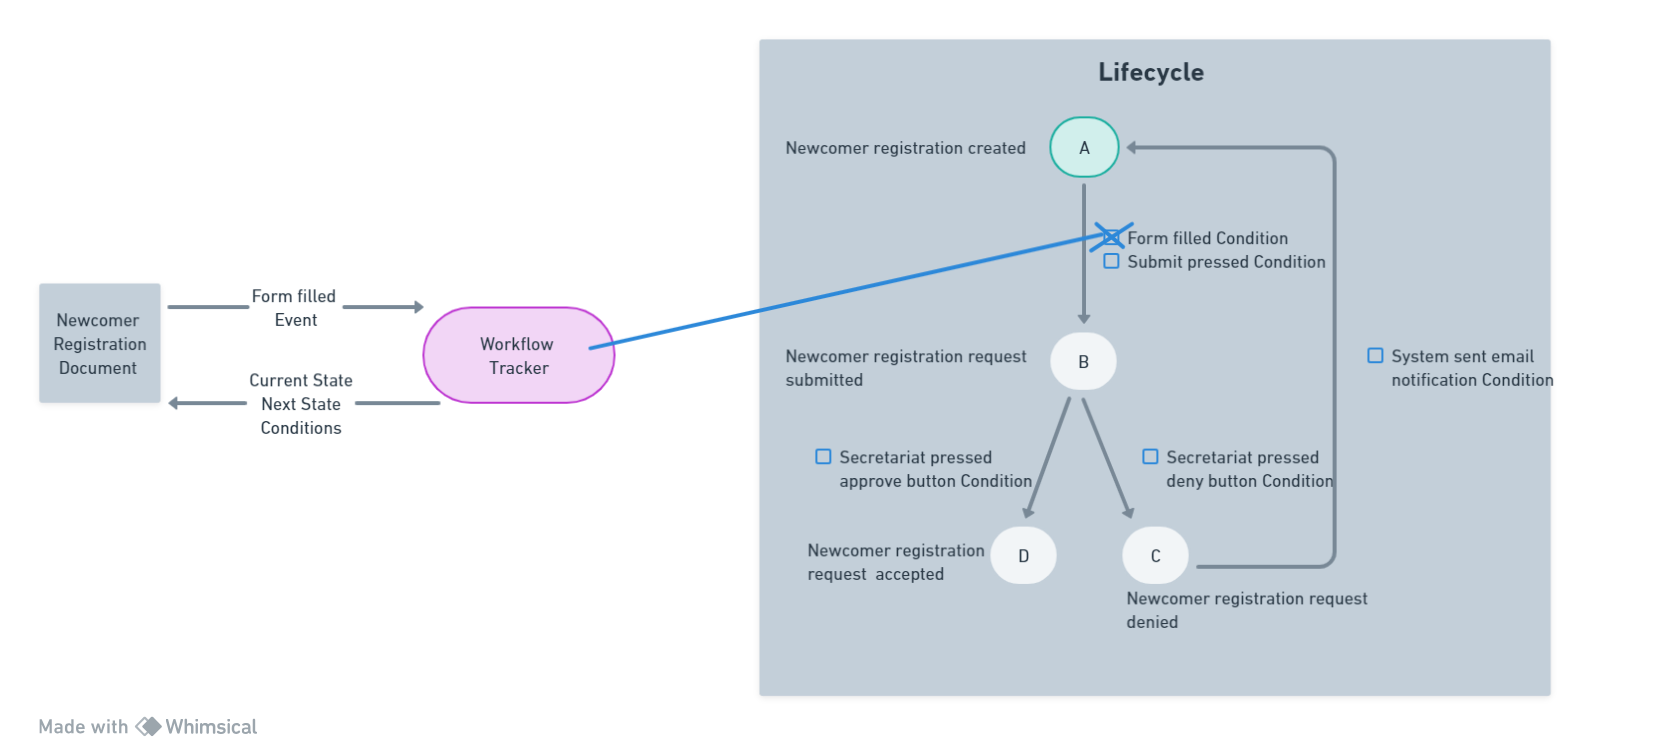
\includegraphics[width=1\linewidth]{figuras/workflow_draft.png}
    \caption{Workflow Tracking Service draft.}
    \label{fig:cap_2_workflow_draft}
\end{figure}

\paragraph{} A more formal version of the draft displayed in Figure \ref{fig:cap_2_workflow_draft} becomes a necessity for the LHCb Analysis Lifecycle Management System (ALCM) \cite{alcm}. This system manages the lifecycle of graphs, such as plots and diagrams, papers, conference notes, and other documents published by the Collaboration. The documents undergo an approval process, involving validation by various Collaboration members based on their appointments. For instance, during parts of the process, the Physics Coordination must approve the document, affirming the content's accuracy. Subsequently, the Editorial Board provides a sign-off, focusing on grammar and formatting. The initial idea was for the ALCM to reuse the same classes created for the Membership Workflow Tracker, but during the planning phase of the project, the developers realized that a more robust solution based on the graph theory would be needed.


\subsection{Discrete-Event Systems}

\paragraph{} A Discrete Event System (DES) can be conceptualized as a mechanism governed by state changes triggered by discrete events. These systems are characterized by a discrete state space and are event-driven. An event refers to any instantaneous occurrence that can lead to a transition in the state of the system. Formally, the set of possible events in a network can be denoted as:
$$
\Sigma=\{p, q\}
$$
where \(p\) represents the arrival of a packet, and \(q\) signifies that the packet queue is full. This scenario encapsulates the dynamism and responsiveness of DES in managing network traffic, where each event (such as the arrival of a new packet or reaching the capacity of a packet queue) precipitates a change in the operational state of the network.

\paragraph{} For a given set \(\Sigma\), its Kleene closure, \(\Sigma^*\), represents the totality of all possible finite-length sequences that can be constructed from the elements of \(\Sigma\), including the empty sequence denoted by \(\epsilon\).

\paragraph{} Example:

\[
\begin{gathered}
\Sigma = \{x, y, z\} \\
\Sigma^* = \{\epsilon, x, y, z, xx, xy, xz, yx, yy, yz, zx, zy, zz, xxx, \ldots\}
\end{gathered}
\]

\paragraph{} This comprehensive collection \(\Sigma^*\) encompasses every conceivable language \(L\) that can be derived from \(\Sigma\), ensuring that \(L\) is either fully contained within or exactly equals \(\Sigma^*\). This includes the specific sets \(\Sigma^*\), \(\Sigma\), and \(\emptyset\). Notably, the empty set \(\emptyset\) is distinct from \(\{\epsilon\}\), which contains a single element, namely the empty sequence \(\epsilon\).

\paragraph{} Consider a sequence \(s = \text{def}\). The segments ``d", ``e", and ``f" of \(s\) correspond to its prefix, subsequence, and suffix, respectively. Therefore, the sequence can be viewed in several relational contexts:
\[
s = s \epsilon, \quad s = \epsilon s, \quad s = \epsilon s \epsilon
\]
In these relations, \(\epsilon\) serves as a universal prefix, suffix, and subsequence for any string, including \(s\).

\noindent 
Example:
\[
s = \text{xyz}
\]
Prefixes of \(s = \{\epsilon, x, xy, xyz\}\). Suffixes of \(s = \{\epsilon, z, yz, xyz\}\).

\paragraph{} In formal language theory, standard set operations such as union, intersection, difference, and complement are applicable to languages since they are sets. For subsets \(L_a\) and \(L_b\) within \(\Sigma^*\), their concatenation is defined as:
\[
L = L_a L_b = \{s = s_a s_b \in \Sigma^* : (s_a \in L_a) \wedge (s_b \in L_b)\}
\]
When considering the prefix closure of a subset \(L\) of \(\Sigma^*\), it is described by:
\[
\bar{L} = \{s \in \Sigma^* : (\exists t \in \Sigma^*)[st \in L]\}
\]
This prefix closure \(\bar{L}\) includes every prefix of every sequence in \(L\). If \(L\) is non-empty, \(\epsilon\) is automatically included in \(\bar{L}\). If \(L\) is empty, then \(\bar{L}\) likewise remains empty. A set \(L\) is prefix-closed if \(L\) and \(\bar{L}\) are identical.

\paragraph{} The Kleene closure of \(L\) further extends this concept:
\[
L^* := \{\epsilon\} \cup L \cup LL \cup LLL \cup \ldots
\]

\noindent
Example:

Consider the alphabet \(\Sigma = \{x, y, z\}\) and two distinct languages \(L_1 = \{\epsilon, x, xyz\}\) and \(L_2 = \{z\}\). Assessing their prefix closures:
\[
\begin{gathered}
\bar{L}_1 = \{\epsilon, x, xy, xyz\} \\
\bar{L}_1 \neq L_1,
\end{gathered}
\]
hence \(L_1\) is not prefix-closed.
\[
\begin{gathered}
\bar{L}_2 = \{\epsilon, z\} \\
\bar{L}_2 \neq L_2,
\end{gathered}
\]
therefore \(L_2\) is not prefix-closed either.

\paragraph{} An automaton is a conceptual model used to represent various types of languages. A deterministic automaton is defined as a sixtuple:
$$
G=\left(X, \Sigma, f, \Gamma, x_0, X_m\right)
$$
where:
\begin{itemize}
  \item \(X\) is the set of states,
  \item \(\Sigma\) is the finite set of events,
  \item \(f: X \times \Sigma \rightarrow X\) is the state transition function, which may be partially defined over its domain,
  \item \(\Gamma: X \rightarrow 2^{\Sigma}\) maps each state to the set of viable (active) events, \(\Gamma(x)\) being the set of active events at state \(x\),
  \item \(x_0 \in X\) is the initial state,
  \item \(X_m \subseteq X\) consists of marked states.
  \item \(L(G)\) is the language generated by the automaton \(G\), consisting of all strings that can be formed by following the transitions starting from the initial state.
\end{itemize}

\paragraph{} A marked state is designated for special significance within the automaton, such as signifying the start of a particular process or the completion of an activity.


\paragraph{} The State Transition Diagram in the context of a deterministic automaton visually represents transitions between states triggered by events as shown in Figure \ref{fig:state_transition_diagram_example}.

\begin{figure} [H]
    \centering
    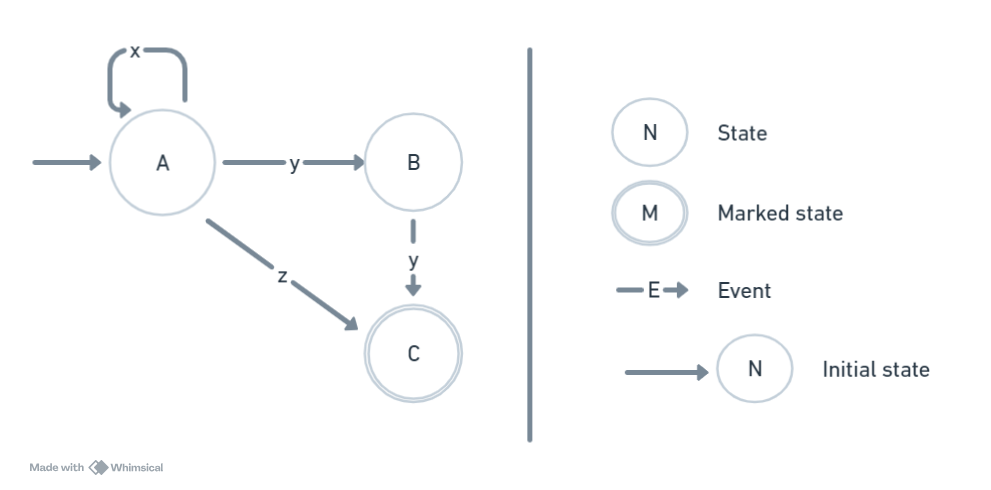
\includegraphics[width=0.7\linewidth]{figuras/automaton.png}
    \caption{State Transition Diagram example.}
    \label{fig:state_transition_diagram_example}
\end{figure}

\noindent
States:
$$
X=\{A, B, C\}
$$

\noindent
Events:
$$
\Sigma=\{x, y, z\}
$$

\noindent
State Function:
For a given state and event, the following function describes the resultant state: \(f(A, x) = A\), \(f(A, z) = C\), \(f(A, y) = B\), \(f(B, y) = C\), \(f(B, x)\) is undefined, \(f(B, z)\) is undefined, \(f(C, x)\) is undefined, \(f(C, y)\) is undefined, and \(f(C, z)\) is undefined.


\noindent
Active Event Function:
This function specifies which events are possible in a particular state:
\[
\Gamma(A) = \{x, y, z\}, \quad \Gamma(B) = \{y\}, \quad \Gamma(C) = \{\}
\]

\noindent
Initial State:
$$
x_0=A
$$

\noindent
Marked States:
$$
X_m=\{C\}
$$

\paragraph{} Figure \ref{fig:state_transition_diagram_example_with_lock} exemplifies the behaviors of locks within state machines, particularly focusing on deadlock and livelock situations. The automaton \(G\) for this figure can be defined as: $G = \left(X, \Sigma, f, \Gamma, x_0, X_m\right)$ where:

\begin{itemize}
  \item \(X = \{A, B, C, D, E, F\}\) is the set of states.
  \item \(\Sigma = \{x, y, v, w, z\}\) is the finite set of events.
  \item \(f: X \times \Sigma \rightarrow X\) is the state transition function, defined by:
  \[
  f(A, x) = A, \quad f(A, y) = B, \quad f(A, v) = F, \quad f(A, w) = D, \quad f(A, z) = C,
  \]
  \[
  f(B, y) = C, \quad f(D, v) = E, \quad f(D, z) = E
  \]
  \item \(\Gamma: X \rightarrow 2^{\Sigma}\) maps each state to the set of viable (active) events, defined as:
  \[
  \Gamma(A) = \{x, y, v, w, z\}, \quad \Gamma(B) = \{y\}, \quad \Gamma(C) = \{\}, \quad \Gamma(D) = \{v, z\},
  \]
  \[
  \Gamma(E) = \{\}, \quad \Gamma(F) = \{\}
  \]
  \item \(x_0 = A\) is the initial state.
  \item \(X_m = \{C\}\) is the set of marked states.
\end{itemize}


\begin{figure}[H]
    \centering
    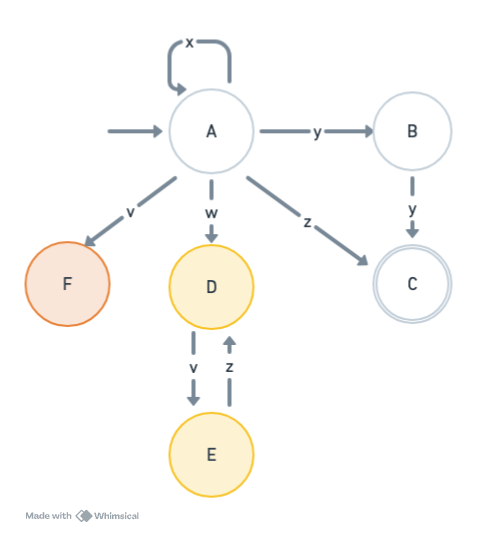
\includegraphics[width=0.5\linewidth]{figuras/automaton_lock.png}
    \caption{State Transition Diagram example with locks.}
    \label{fig:state_transition_diagram_example_with_lock}
\end{figure}

\paragraph{} State F represents a deadlock condition, characterized by the absence of any possible events that could trigger a transition from this state. Once reached, the system remains indefinitely in this state, unable to progress to a marked state. States D and E together demonstrate a livelock scenario. While there are events that transition the system between these two states, no event leads to a marked state.

\paragraph{} A system experiences a blocking when the following condition is met:
$$
\overline{L_m(G)} \subset L(G)
$$
\noindent
Conversely, there is no blocking within the system when:
$$
\overline{L_m(G)}=L(G)
$$



\paragraph{} The generated language \(L(G)\) includes: \(x^n\) (staying in \(A\) via \(x\)), \(x^n y\) and \(x^n y y\) (from \(A\) to \(B\) and then to \(C\)), \(x^n z\) (from \(A\) to \(C\)), \(x^n v\) (from \(A\) to \(F\)), \(x^n w v\) (from \(A\) to \(D\) to \(E\)), \(x^n w v z\) (from \(A\) to \(D\) to \(E\) and back to \(D\)). It can also loop between \(D\) and \(E\). Hence:
\[
L(G) = \left\{ x^n, x^n y, x^n y y, x^n z, x^n v, x^n w, x^n w v, x^n w v z, x^n w v z v, x^n w v z v z ... \mid n \geq 0 \right\}
\]
The marked language \(L_m(G)\) consists of strings that end in the marked state \(C\):
\[
L_m(G) = \left\{ x^n y y, x^n z \mid n \geq 0 \right\}
\]
The prefix-closure \(\overline{L_m(G)}\) includes all prefixes of strings in \(L_m(G)\):
Prefixes of \(x^n y y\): \(\left\{ \epsilon, x, x^2, \ldots, x^n, x^n y, x^n y y \right\}\)
Prefixes of \(x^n z\): \(\left\{ \epsilon, x, x^2, \ldots, x^n, x^n z \right\}\)
Thus:
\[
\overline{L_m(G)} = \left\{ x^m, x^m y, x^m y y, x^m z \mid m \geq 0 \right\}
\]
Checking for locks using the conditions provided:
Lock Condition: \(\overline{L_m(G)} \subset L(G)\)
\[
\overline{L_m(G)} = \left\{ x^m, x^m y, x^m y y, x^m z \mid m \geq 0 \right\}
\]
\[
L(G) = \left\{ x^n, x^n y, x^n y y, x^n z, x^n v, x^n w, x^n w v, x^n w v z, x^n w v z v, x^n w v z v z ... \mid n \geq 0 \right\}
\]
Since \(\overline{L_m(G)}\) does not include strings with \(v\), \(w v\), or \(w v z\), and these strings are part of \(L(G)\), it is evident that:
\[
\overline{L_m(G)} \subset L(G)
\]

\noindent
Given that \(\overline{L_m(G)}\) does not include all strings from \(L(G)\), the condition \(\overline{L_m(G)} = L(G)\) is not met.

